\documentclass[10pt]{article}
\usepackage[margin=23mm]{geometry}
\usepackage{amsmath,amssymb,booktabs,graphicx,longtable,array}
\usepackage[T1]{fontenc}
\usepackage{lmodern}
\usepackage[hidelinks]{hyperref}
\newcommand{\Qf}{\mathsf Q}
\title{Reproducibility Supplement\\
\large Target-Local Fusion for Communication-Efficient Multi-UAV OTFS-ISAC Sensing}
\author{Technical revision accompanying the five-page manuscript}
\date{16 September 2026}
\begin{document}
\maketitle
\noindent This supplement supplies derivations and implementation details without
adding a new sensing mechanism. The main results are the V1 experiments,
regenerated in full under the current frozen release so that the reported
numbers and the code that produces them agree. New component audits are
labeled separately and do not replace the
1000-trial comparison. File paths below are relative to the repository root.

\section{Reporting semantics and information available to the scheduler}
Observation $(i,j,q)$ is produced at echo receiver $j$, following
$i\to q\to j$. It is either consumed locally when $j=f_q$ or transmitted on
$j\to f_q$. All selected statistics for a target have one destination.
Different targets can have different destinations. The reporting view uses
the source and destination to obtain rate, success probability, and cost;
these quantities are not attributes of the sensing pair $i\to j$.

The task begins after acquisition. The simulated tracker output perturbs
horizontal position by independent Gaussian errors with standard deviation
150 m and horizontal velocity by 15 m/s. Actual altitude is retained and
vertical velocity is zero in this simulator. The supplied covariance is a
six-coordinate diagonal proxy with the same position/velocity variance on
each axis, including conservative nonzero vertical entries. It is not a
calibrated posterior from an implemented tracker. The delay/Doppler gate uses
the bistatic Jacobian applied to this covariance and a three-standard-deviation
margin in each coordinate. Selection uses the predicted geometry and mean
RCS of $50~\mathrm{m}^2$ at the nominal work point, and $0.1~\mathrm{m}^2$ at
the low-RCS work point of Sec.~\ref{sec:work_points}; detection uses the unknown
current state. At the low-RCS work point the declared 150~m position error
exceeds one delay-resolution cell (78.1~m for $L=64$ and
$\Delta f=30$~kHz), which is why the belief-error term discussed there matters
and why the two work points are never mixed in one table. Blind first
acquisition and inference of an unknown target inventory are outside scope.
The position-error scan tests 50--500 m; it does not prove robustness to arbitrary
tracking errors or unknown RCS distributions.

Sensing and communication share power and propagation. Reports are orthogonal
and serial, while continuous sensing components cause residual leakage in the
communication SINR. The complex AWGN normal approximation is applied
conditionally to that effective SINR. It is a packet-success abstraction,
not a specific decoder's measured block-error curve. In particular, it does
not derive the failed-soft-report distribution.

The remaining nominal parameters are listed below; the archived resolved JSON
is authoritative for inactive legacy fields.
\begin{center}\small
\begin{tabular}{ll}
\toprule
Quantity & Value or convention\\
\midrule
Receiver noise & $-174$ dBm/Hz PSD; 7 dB noise figure\\
Communication fading & Rician $K=15$ dB; lognormal shadowing SD 1 dB\\
Communication path-loss exponent & 2\\
Sensing processing / hardware gain & $G_p=NL=4096$; $G^{\rm hw}=1$\\
Direct-path cancellation in sensing & 40 dB\\
Residual sensing leakage into reports & 0.05; desired-source leakage factor 0\\
Residual self-sensing power factor & $10^{-14}$\\
Numerical SINR guard & $10^{-3}$ times receiver noise power\\
Minimum remote success probability & 0.3\\
UAV / target height ranges & 800--1200 m / 700--1500 m\\
\bottomrule
\end{tabular}
\end{center}
The sensing field includes the illuminator's direct path and other continuously
radiating UAVs, attenuated by the stated cancellation. Reporting packets are
absent during the sensing observation phase. These coefficients define a
simulation operating point; they are not calibrated measurements.

\section{DD computation and probability model}
\subsection{Finite-grid local energy}
Let $\ell=\tau L\Delta f$ and $\kappa=\nu NT$.
For either axis with length $A$, evaluate
\[
 p_A(b;z)=
 \frac{\left|\sin(\pi(b-z))/[A\sin(\pi(b-z)/A)]\right|^2}
 {\sum_{a=0}^{A-1}\left|\sin(\pi(a-z))/[A\sin(\pi(a-z)/A)]\right|^2}.
\]
The implementation wraps differences to the periodic grid, handles a vanishing
denominator by continuity in magnitude, and normalizes the squared magnitudes.
It caches fractional centers to $10^{-3}$ bin. Sum
$p_N(b;\kappa)p_L(d;\ell)$ for the nine wrapped bins centered on
$(\operatorname{round}\kappa,\operatorname{round}\ell)$ to obtain
$\eta^{\rm loc}$. This is a fraction of total impulse-response energy and
therefore lies in $[0,1]$. The fine gain is exactly this fraction in V1.
Legacy interpolation and floor parameters are inactive. The coarse
$\mathrm{sinc}^2$ product approximates finite-grid center-bin energy; it is
not exactly the finite-$A$ Dirichlet energy at window radius zero.
$W=1$ fixes a small processing window; the manuscript does not claim it is optimal.

This separable model is checked against the compact OTFS modulation/channel/
demodulation kernel implemented in \texttt{isac\_sim/waveform.py}. That check
does not establish a general input--output law with arbitrary pulses, CP,
multipath, synchronization errors, or coherent multi-target interference.
The rounded-bin collision penalty $1/n_{ijq}$ remains an occupancy surrogate.

\subsection{Exact mixture moments, approximate detection}
For $K$ independent looks, $X\mid H_h\sim\operatorname{Gamma}(K,1+h\gamma)$.
The centered statistic $\ell=\gamma(X-K)/(1+\gamma)$ differs from the
energy-detector LLR by a hypothesis-independent constant. Its null mean is
zero and its alternative mean and variances are
\[
 \delta=\frac{K\gamma^2}{1+\gamma},\qquad
 v_0=\frac{K\gamma^2}{(1+\gamma)^2},\qquad v_1=K\gamma^2 .
\]
Assume delivery $A\sim\operatorname{Bernoulli}(\chi)$ is independent of the
local statistic conditional on the modeled state and channel. Set
$Y=A\ell+(1-A)Z$, where $Z\sim{\cal N}(0,av_0)$ is independent.
The law of total expectation gives $E[Y\mid H_1]=\chi\delta$.
The conditional-variance identity gives
\[
 \operatorname{Var}(Y\mid H_h)
 =\chi v_h+(1-\chi)av_0+\chi(1-\chi)(h\delta)^2 .
\]
Thus the calibration is exact under this explicitly specified mixture;
omitting the between-component term under $H_1$ would be incorrect.
For the centered-Gamma null, the third central moment is
$\chi\,2K[\gamma/(1+\gamma)]^3$, since the replacement Gaussian has zero third
moment. Independent weighted sums add means, variances, and third cumulants.
Their standardized null skewness supplies the first-order Cornish--Fisher
correction used in the archived V1 threshold.

The Q-function detection prediction based on these moments remains
approximate. Exact first and second moments do not make the received
distribution Gaussian. Independent observations and known modeled SINRs
are assumptions, not consequences of shared illumination.

\subsection{Historical error-model naming: essential reproduction detail}
The archived configurations in \texttt{results\_target\_local\_v1} name the
failure model \texttt{erasure}. At source revision \texttt{69f3300}, which
records the main result configuration, that branch in
\texttt{isac\_sim/soft\_channel.py} actually draws zero-mean Gaussian
replacement with variance $9v_0$. The corresponding detector uses the
Cornish--Fisher threshold for all methods. Hence the main manuscript
correctly describes $a=9$, not zero-valued erasure.

The current code distinguishes \texttt{gaussian\_replacement} ($a=9$) from
\texttt{erasure} ($a=0$). Current true-erasure evaluation additionally uses
a calibrated mixture null threshold. Loading the old JSON unchanged into
current code therefore changes the experiment. The V1 rerun tool now
explicitly selects \path{detect.comm_error_model=gaussian_replacement}.
This maps the failure semantics; it is not a claim that all current source
changes reproduce historical detection draws bit for bit. Archive data are
preserved. A full replacement of the headline evidence requires a new paired
main run, not relabeling an audit. That rerun has since been performed: the
regenerated tree reproduces every selection-path quantity of the archived tree
bit for bit (deflection, selected observations and reports, payload, serial
delay, refinement counts, belief capture), while the detection counts move by
at most 0.0003 in $P_D$ at 1000 trials. That signature is the sampling-path
change alone and not a changed physical or optimisation model.

\section{Conditional guarantees and algorithm boundary}
\subsection{What local delivery guarantees}
For one fixed observation with $\delta>0$ and $v_0>0$, its post-report
deflection is
\[
 d(\chi)=\frac{\chi^2\delta^2}{v_0[a+(1-a)\chi]}.
\]
For positive denominator,
\[
 d'(\chi)=\frac{\delta^2}{v_0}
 \frac{\chi[2a+(1-a)\chi]}{[a+(1-a)\chi]^2}\ge0,
 \qquad 0<\chi\le1,\quad a\ge0.
\]
For $a>1$, the bracket is at least $a+1$; for $0\le a\le1$ it is nonnegative.
The boundary $a=\chi=0$ is defined by the zero-information limit.
Local delivery ($\chi=1$) therefore maximizes this single-observation
deflection and avoids its packet. This theorem holds the observation fixed.
It neither proves monotonicity of approximate detection nor says that
moving a target's fusion destination improves all other reporting links.

For a fixed selected set $S_q$, define
$a_{qm}=|\{(i,j,q)\in S_q:j=m\}|$. Then
\[
 N_{{\rm rem},q}(m)=|S_q|-a_{qm}
 \ \ge\ |S_q|-\max_{u\in{\cal M}}a_{qu}.
\]
Each selected observation requires one report except those received at the
chosen fusion node, which proves the identity and bound. Among feasible
destinations, maximizing $a_{qm}$ minimizes reports for this fixed set.
Nearest-target placement is certified only when it is feasible and attains
that bound. There is no claim that it does so in every scenario.

A separate experimental fixed-set destination search checks predicted
per-target detection floors and reporting feasibility in decreasing $a_{qm}$
order. With no coupled destination capacities, the first feasible destination
is report-minimal under those fixed-set constraints. It does not solve joint
observation selection. This candidate remains outside the main paper:
nominal held-out report reductions were small, and lower predicted loss is
not a guarantee on true detection. See
\texttt{V1\_FUSION\_THEORY\_AND\_ALGORITHM.md} for that separate audit.

\subsection{Objective, budgets, and reproducible selection rules}
The main paper provides the exact capped weak-target utility, the remote
delay price, and pseudocode for coarse selection and fine replay.
Soft-min temperature is 0.1, gap coefficient is 1, and the price is
0.005 per millisecond. Both utility terms are retained to match archived
experiments; an independent ablation identifying the need for both has not
been completed. They are design choices, not separate novelty claims.

The admissible set requires DD validity and either a local receiver or a
remote link satisfying range, rate, and reliability checks.
Caps are six observations per target and 60 overall, including local
observations. These are not prescribed hard communication constraints.
A fixed packet contains 640 reserved payload bits and occupies
$2048/(64\cdot30\,000)=1.0667$ ms. Thus the loose implied bounds are
38.4 kbit and 64 ms. The reported 83.7\% reductions share the same cause:
fewer packets. They are not independent gains. Header overhead, control
exchange, route discovery, retransmission, packet aggregation, and processing
time are excluded. No bit-level quantizer or implemented packet format is
validated by the four-times-160-bit reservation.

\begin{center}
\small
\begin{tabular}{p{30mm}p{64mm}p{49mm}}
\toprule
Method & Selection & Resource relationship\\
\midrule
Target-local adaptive C2F &
Nearest predicted fusion; positive detector-utility minus delay marginal;
coarse frontier and fine replay &
Six per target, 60 total; remote count is an outcome\\
Sensing-SINR &
Descending coarse sensing SINR on the same feasible reporting graph &
Matches V1's per-target observation counts; remote reports need not match\\
Exact-marginal greedy &
Greedy deflection-utility marginal; no delay price; no adaptive replay &
Total count capped at V1's realized count; six per target; positive-gain
stopping can use fewer\\
Full-refinement PD control &
Same priced detector-utility rule after refining all feasible candidates &
Same configured caps, without forcing realized count equality; not an oracle\\
All-neighbor reference &
All feasible observations &
Upper-resource diagnostic only; not a matched-budget detection upper bound\\
\bottomrule
\end{tabular}
\end{center}

The frontier cap is $J=25$ per target. Coarse and fine greedy stages both check
caps, require positive deflection increment, and stop at no positive objective
gain. The fine stage resets the selected set. The method does not use a
certified upper bound for omitted candidates, and therefore cannot claim
lossless screening or a universal greedy approximation ratio.
At most $L_{\rm tot}$ commits per stage require
$O(L_{\rm tot}(E+r))$ candidate scores. A direct score costs
$O(L_{\max}+Q)$ for moments and target utility; caching can reduce this.
DD work is $EC_c+rC_f$, with $r\le E$ and frontier storage at most $QJ$.
The current simulator precomputes fine DD arrays in shared table construction:
counted refinement savings alone are not evidence of end-to-end runtime savings.

\section{Additional validation and evidence inventory}
\subsection{New component audit, separate from the headline trials}
The command is
\begin{quote}\small\ttfamily
python tools/audit\_isac\_review\_revision.py\\
--error-model gaussian\_replacement\\
--out results\_isac\_review\_revision --runtime-trials 30
\end{quote}
The stored protocol records configuration, source hashes, Python and NumPy,
and CPU identifier. The machine uses an AMD Ryzen 7 7800X3D.
The DD audit uses 512 offsets (seed 913). Six single-report waveform-derived
LLR cases use raw SINR 0.5 or 2 and delivery probability 1, 0.7, or 0.3,
each with $10^5$ draws (seed 914), 16 looks and fractional offset
$(0.31,-0.27)$. They assume the compact isolated-target waveform without
added multipath, synchronization error, or multi-target interference.
The report success coin is imposed, not produced by a channel decoder.

\begin{center}
\begin{tabular}{lr}
\toprule
Audit quantity & Observed maximum discrepancy\\
\midrule
Local-window energy vs compact OTFS impulse response & $3.11\,10^{-15}$\\
Coarse sinc energy vs impulse response & $1.057\,10^{-3}$\\
Exact single-report mixture $P_D$ vs sampled waveform statistic & 0.00184\\
Exact mixture $P_{\rm FA}$ vs sampled waveform statistic & 0.000667\\
Moment-predicted $P_D$ vs sampled waveform statistic & 0.04465\\
Mixture variance relative sampling discrepancy & 0.735\%\\
\bottomrule
\end{tabular}
\end{center}

The mixture audit separately uses $2\,10^5$ samples per hypothesis and
parameter combination, delivery probabilities 0.3, 0.7, 1 and replacement
standard-deviation factors 0, 1, 3 (seed 915). Its largest mean discrepancy
is 1.505 standard errors. These checks verify the mixture identity under
simulation, not the appropriateness of Gaussian replacement for a deployed
decoder.

For example, at raw SINR 0.5 and $\chi=1$, moment prediction is 0.46930,
the exact mixture probability at the implemented threshold is 0.43649,
and empirical detection is 0.43547 with 95\% Wilson interval
$[0.43240,0.43855]$. This counterexample rules out treating moment alignment
as exact detection prediction.

A separate zero-replacement audit is stored under
\texttt{results\_isac\_review\_revision\_erasure}. Its maximum moment-prediction
error is 0.31343, versus 0.00103 for exact mixture detection. It tests the
Cornish--Fisher component predictor with true erasures, not the current
system's separately calibrated erasure detector. This is a limitation of
transferring the scheduling approximation to an atom-at-zero distribution,
and is not inserted into the main V1 results.

\subsection{Selector timing and uncertainty}
Thirty new scenarios use seed sequence $[916,t]$, after one warm-up scenario.
Adaptive and full-refinement calls alternate order within each scenario and
use shared belief-side tables. Median selector times are 0.5556 and 2.0324 s;
means are 0.6296 and 2.2547 s. Mean fine-evaluation counts are 64.5 and 882.
The ratio of medians is 3.66, not an end-to-end system speedup.
Shared geometry generation, channel construction, and precomputed fine arrays
are excluded. No parallel worker pool is used by this timing script.
Per-trial times are retained in \texttt{selector\_runtime.csv}; waveform
Wilson intervals are retained in \texttt{waveform\_llr.csv}.

Archived headline $P_D$ bars are pooled Wilson intervals. They do not model
within-scenario target dependence; the paired method-difference intervals
are the relevant comparison reported in the main text. A confidence interval
crossing zero is not proof of equivalence or non-inferiority. The regenerated
V1 active-target false-alarm estimate is 0.04868, near the specified 0.05.
This aggregate observation does not guarantee exact false-alarm control
for every selected set or every operating condition.

\subsection{Source data and supplementary scans}
\begin{itemize}
\item \texttt{results\_target\_local\_v1/main/main.csv}: regenerated 1000-trial main comparison.
\item \texttt{results\_target\_local\_v1/full-refinement-pd}: 200-trial computational control.
\item \texttt{results\_target\_local\_v1/overview}: 100-trial fusion and parameter scans.
\item \texttt{results\_target\_local\_v1/prediction-stress}: position-belief scan.
\item \texttt{results\_isac\_review\_revision}: new Gaussian-replacement component audits.
\item \texttt{results\_isac\_review\_revision\_erasure}: separately labeled zero-replacement audit.
\end{itemize}
The two main result figures remain in the five-page manuscript. The six-panel
operating envelope is placed here to keep its diagnostic role distinct.
Changing deployment side length and fleet size does not isolate an independent
density law. Price, rate, and blocklength scans are calibration evidence, not
new algorithmic contributions.

\begin{figure}[htbp]
\centering
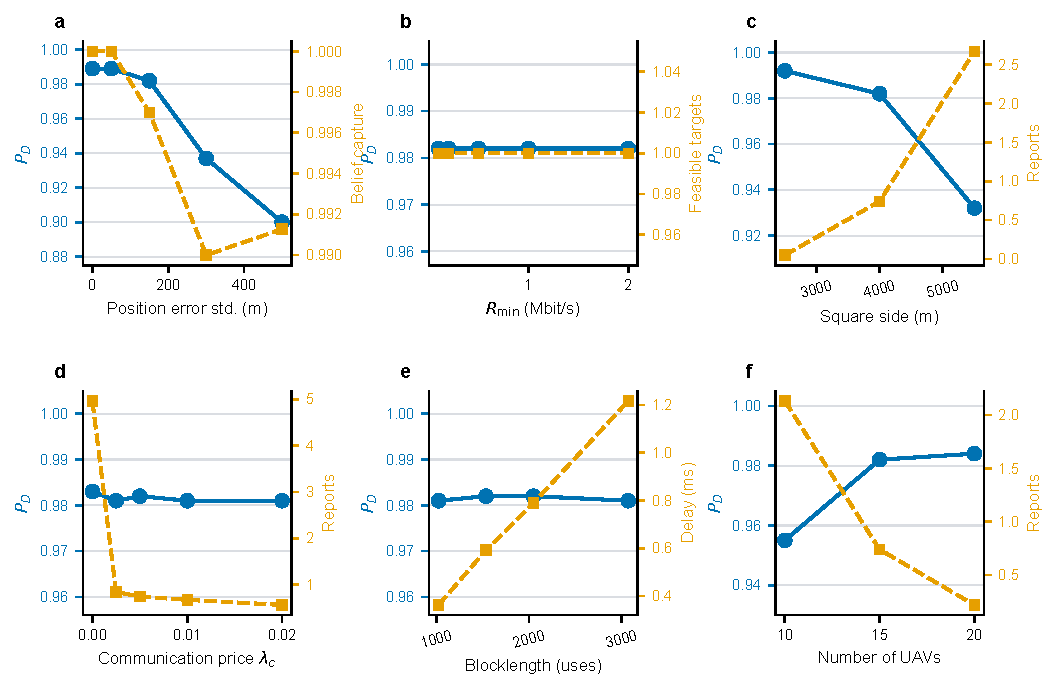
\includegraphics[width=\linewidth]{figs/fig4_v1_operating_envelope.pdf}
\caption{Operating envelope, 100 trials per condition.
(a) Position-belief error, (b) minimum reporting rate, (c) deployment side,
(d) communication price, (e) blocklength, (f) fleet size. Blue denotes
detection probability and orange the named secondary metric.
No additional uncertainty bands are shown for these diagnostic scans.}
\end{figure}
\clearpage
\section{Stronger detection guarantee and probability refinement}
\subsection{Optimal ROC dominance for a fixed observation law}
Fix the local observation law $P_h$ under hypothesis $h\in\{0,1\}$ and a
replacement law $G$ independent of the hypothesis. A received report has law
$Q_{h,\chi}=\chi P_h+(1-\chi)G$. For
$0\le\chi_1\le\chi_2\le1$ and $\chi_2>0$, keep a report with success $\chi_2$
with probability $\alpha=\chi_1/\chi_2$, otherwise generate an independent
draw from $G$. The output law is
\[
 \alpha Q_{h,\chi_2}+(1-\alpha)G
 =\chi_1P_h+(1-\chi_1)G=Q_{h,\chi_1}.
\]
This transformation is independent of $h$. Any randomized test on the
less reliable report can be simulated from the more reliable one with the
same false-alarm and detection probabilities. Writing $\beta^*(u;\chi)$
for maximum detection over tests with false-alarm probability at most $u$,
\[
 \beta^*(u;\chi_2)\ge\beta^*(u;\chi_1),\qquad 0\le u\le1.
\]
The zero-success boundary is trivial. For independent report coordinates,
apply the transformation coordinate by coordinate under componentwise
larger success probabilities.

This applies statistical experiment degradation (D. Blackwell, 1953,
\href{https://doi.org/10.1214/aoms/1177729032}{doi:10.1214/aoms/1177729032});
it is not a new general detection theorem. It strengthens the deflection
argument to the optimal ROC envelope. It does not prove monotonicity for
a fixed linear/CF detector, nor for moving a fusion destination when other
reports become less reliable. Each observation's replacement law must
remain fixed and hypothesis-independent. Biased or sign-flip failure
models are not covered.

\subsection{Distribution evaluation without Gaussian moment matching}
For a fixed independent set and fixed weights, each weighted input mixes
a shifted, scaled Gamma variable with a Gaussian (or a zero atom).
The single-report tail follows directly from their CDFs. For multiple
inputs, the audit computes bin masses from these CDFs and convolves them.

Choose common spacing $h$ and a finite retained range for each $X_e$.
On the retained event $B$, its rounded-down value $L_e$ satisfies
$L_e\le X_e<L_e+h$. For $s$ inputs,
$L=\sum_eL_e\le T=\sum_eX_e<L+sh$. The unnormalized convolution retains
the probability of $B$, rather than discarding the tail mass. Hence
\[
 \Pr(L>t,B)\le\Pr(T>t)
 \le\Pr(L+sh>t,B)+\Pr(B^c).
\]
Range endpoints use component quantiles and union tail budget $10^{-9}$.
The implementation halves $h$ until bracket width is at most $10^{-3}$
or the 262144-bin limit binds, returning unresolved status in the latter case.
Zero atoms use the strict rule $T>t$.

These inequalities hold for exact bin masses and convolution.
SciPy CDFs and FFT convolution use a monitored roundoff allowance, not
formally certified interval arithmetic. The brackets exclude uncertainty
in belief, SINR, independence, and the failed-report model.

The adapter evaluates the existing CF-threshold statistic on supplied
belief-side tables, without changing observations or main results.
A future acceptance check can require the new probability's lower bound
to exceed the incumbent's upper bound. Overlap requires further refinement
or an unresolved decision. This protects the specified model comparison,
not unknown truth.

\subsection{New checks and computational placement}
Run \path{tools/audit_probability_refinement.py}; results are in
\path{results_v1_probability_refinement}.
For the six saved Gaussian-replacement waveform cases at their original
thresholds, maximum discrepancy from empirical detection changes from
0.04464 for moment prediction to 0.00184 for direct mixture tails.
The latter matches the analytic singleton reference within $4.45\,10^{-16}$;
its empirical discrepancy includes sampling noise.

Twelve new synthetic sets contain two, three, or six observations,
six sets each for $a=9$ and $a=0$. SINRs are uniform on $[0.08,0.65]$,
success probabilities on $[0.3,1]$, with seed sequence $[10217,r]$ and
200000 Monte Carlo draws per set. All brackets converge, with maximum
width 0.000864. Maximum discrepancy from empirical rates is 0.00271,
versus 0.06063 for moment prediction. Empirical differences are not
deterministic integration-error bounds. Median tail evaluation takes
0.0178 s for these sets.

Eight nominal V1 scenarios (seed sequence $[10218,r]$) supply 80 selected
target sets. All detection and false-alarm brackets converge at the requested
tolerance. Median two-hypothesis audit time is 0.000260 s per target;
many nominal sets are singletons. The largest change from old predicted
$P_D$ is 0.01859. These are belief-side model evaluations, not a new
detection-performance experiment.

The current use is final-set verification and inspection of close decisions.
Convolution inside every coarse greedy score would change runtime and
requires a separate benchmark. Released C2F and the MC=1000 headline are
unaffected by this verification path.

\subsection{Novelty boundary after targeted literature search}
Primary versions checked include Chen et al.'s shared-backhaul selection
(arXiv:2405.16791), Li et al.'s limited-backhaul sensing (arXiv:2404.03440),
Ge et al.'s target handover (arXiv:2411.01871), and Bai et al.'s
belief-propagation handover (arXiv:2506.23118). Backhaul-aware selection and
target-dependent information exchange are therefore prior art.
Our narrower focus is pre-report local/remote classification for bistatic
OTFS observations and its coupling to detector-aligned adaptive C2F.
ROC dominance and numerical convolution are supporting tools, not new
general algorithms.

Per-paper distinctions and search limitations are recorded in
\path{V1_THEORY_PROBABILITY_NOVELTY_UPGRADE.md}.
This targeted review is not an exhaustive novelty certification.

\end{document}
